\documentclass{article}

\usepackage{geometry}
\geometry{
    a4paper,
    total={210mm,297mm},
    left=20mm,
    right=20mm,
    top=20mm,
    bottom=20mm
}

\usepackage[utf8]{inputenc}
\usepackage[english]{babel}
\usepackage[T1]{fontenc}
\usepackage{booktabs}
\usepackage{graphicx}
\usepackage{hyperref}
\usepackage{amsmath}
\usepackage{amsfonts}
\usepackage{tikz}
\usepackage{nameref}
\usepackage{algorithm}
\usepackage{stmaryrd}
\usepackage{listings}
\usepackage{color}
\usepackage{enumitem}
\usepackage{mathtools}
\usepackage{textcomp}
\usepackage{lscape}
\usepackage{pbox}
\usepackage{url}

% enable footnotes in tables
\usepackage{footnote}
\makesavenoteenv{table}
\makesavenoteenv{tabular}

% https://en.wikibooks.org/wiki/LaTeX/Source_Code_Listings#Settings
\lstdefinestyle{customc}{
    belowcaptionskip=1\baselineskip,
    breaklines=true,
    %frame=L,
    numbers=left,
    numberstyle=\tiny,
    xleftmargin=\parindent,
    language=C,
    showstringspaces=false,
    basicstyle=\footnotesize\ttfamily,
    keywordstyle=\bfseries\color{green!40!black},
    commentstyle=\itshape\color{purple!40!black},
    identifierstyle=\color{blue},
    stringstyle=\color{orange},
}
\usepackage{algpseudocode} %https://en.wikibooks.org/wiki/LaTeX/Algorithms#Typesetting_using_the_algorithmicx_package
%\usepackage[labelformat]{caption}

% define figure and table caption numbering
\renewcommand{\thefigure}{\arabic{section}.\arabic{figure}}
\renewcommand{\thetable}{\arabic{section}.\arabic{table}}

% reset counter for figures and tables in each section
\makeatletter
\@addtoreset{figure}{section}
\@addtoreset{table}{section}
\makeatother

\graphicspath{ {images/} }
%\setlength{\parindent}{0in}

\newcommand{\gqm}[1]{\glqq #1\grqq}

\newcommand{\clicommand}[1]{\\[2mm]\texttt{#1}\\[4mm]}

\newcommand{\ownref}[1]{(see \ref{#1} \nameref{#1}, p.\,\pageref{#1})}

\urldef\twoscomplementwikiurl\url{https://en.wikipedia.org/wiki/Two%27s_complement}

\begin{document}

\begin{center}
{\Huge\bfseries Documentation}\\[2mm]
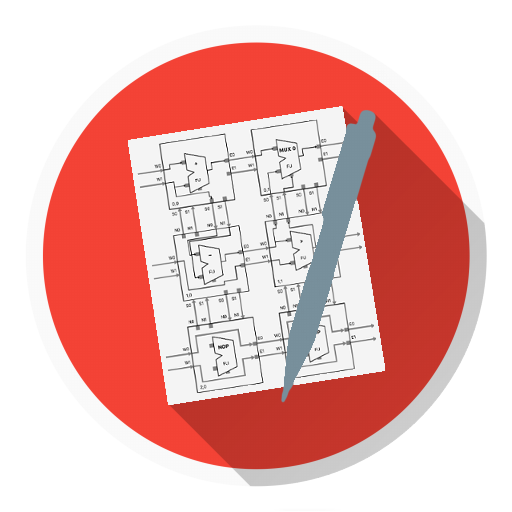
\includegraphics[width=0.2\textwidth]{../idea/src/icon/icon_512x512.png}\\[3mm]
{\Huge\bfseries CRC Configurator}\\[2mm]
Konstantin Lübeck, \today
\end{center}

\noindent This document serves as documentation for the CRC Configurator.\\

\hfill\textit{If in doubt, use the source Luke.}

\section*{Requirements}
\begin{itemize}
    \item \texttt{Java 1.8.0\_40} or higher
    \item IntelliJ IDEA CE 2016.1 or higher
\end{itemize}

\section*{Compile}
After cloning the repository from gitlab one has to compile the program into a \texttt{*.jar}. This is done by using IntelliJ IDEA CE 2016. 
\begin{enumerate}
    \item Open IntelliJ and click on \textit{Import Project}
    \item Choose the directory \texttt{idea} from the cloned repository and click on \textit{OK}.
    \item Choose \textit{Create project from existing sources} and click on \textit{Next}.
    \item Set an appropriate \textit{Project Name} (\texttt{crc\_configurator}), make sure the file path is set to \texttt{crc\_configurator/idea}, and click on \textit{Next}. (Overwrite \texttt{.idea} when asked)
    \item Click on \textit{Next} two times in the library dialog. (Overwrite \texttt{idea.iml} when asked)
    \item Choose the SDK (\texttt{Java 1.8.0\_40} or higher) and click on \textit{Next}.
    \item Click on \textit{Finish}.
    \item Go to menu \textit{File $\rightarrow$ Project Structure}.
    \item Choose the \textit{Artifacts}.
    \item Click on the \textit{+}-sign.
    \item Choose \textit{JAR $\rightarrow$ From modules with dependencies}.
    \item Click on \textit{OK} in the \textit{Create JAR from Modules} dialog.
    \item Click on \textit{OK} in the \textit{Project Sturcture} dialog.
    \item Go to menu \textit{Build $\rightarrow$ Build Artifacts\dots}
    \item Choose Action \textit{Build}.
    \item Open a terminal and navigate to the cloned git repository.
    \item In the git repository go to \texttt{idea/out/artifacts/idea\_jar}
    \item Rename the \texttt{idea.jar} to \texttt{crc\_configurator.jar}.
    \item Copy the \texttt{crc\_configurator.jar} to a desired location.
\end{enumerate}

\section*{Run}
Go to the location of the \texttt{crc\_configurator.jar} and execute the following command:\\[2mm]
\texttt{java -jar crc\_configurator.jar}\\[2mm]

\section*{Usage}
\subsection*{New File}

To open a new CRC description file go to menu \textit{File $\rightarrow$ New}. Set values for \textit{Rows}, \textit{Columns}, \textit{Static Conf. Lines}, and \textit{Dynamic Conf. Lines}, and click on \textit{Create} to create the new CRC description file.
\subsection*{Set FU Functions}

To set the possible FU functions for each PE go to the \textit{Hardware Model} tab. Open the FU functions dialog for a PE by double clicking on the PE's FU. Check the checkboxes of the desired functions and click on \textit{Save}. The enabled FU functions can be seen below each PE in the \textit{Hardware Model} tab.

\subsection*{Configure a CRC}
To create a configuration for a CRC choose one of the \textit{Static Configuration} or \textit{Dynamic Configuration} tabs. To choose a FU operation for a PE right click or double click on the name of the operation in the FU (default \textit{NOP}). To choose  if the FU should treat values as signed or unsigned right click or double click on signed/unsigned (default unsigned). To set the driver for a FU input or a PE output right click or double click on the gray pad next to the FU or arrows and choose a driver. To set no driver click on the checked item in the context menu while choosing a driver.

\subsection*{Edit a CRC}
To change the dimensions (rows and columns) or the amount for static and dynamic configuration lines go to menu \textit{File $\rightarrow$ Edit}. Set the desired values for \textit{Rows}, \textit{Columns}, \textit{Static Config. Lines}, and \textit{Dynamic Config. Lines} and click on \textit{Apply}. \textbf{Caution:} If a value is decreased data will be lost.

\subsection*{CRC/PE Configuration Bits}
To get the CRC/PE configuration bits go to menu \textit{File $\rightarrow$ Export Bits}. The \textit{Export Bits} dialog displays the bits for the Verilog parameters.

\end{document}
